\documentclass[11pt,a4paper]{article}

\usepackage[left=2cm,text={17cm, 24cm},top=3cm]{geometry}
\usepackage[czech]{babel}
\usepackage[utf8]{inputenc}
\usepackage{times}
\usepackage{graphicx}
\usepackage{picture}
\usepackage[longend,ruled,linesnumbered,noline,boxed,czech]{algorithm2e}
\usepackage{algorithmic}
\usepackage{float}

\renewcommand{\algorithmicrequire}{\textbf{Input:}}
\renewcommand{\algorithmicensure}{\textbf{Output:}}

\begin{document}

\begin{titlepage}
\begin{center}
	\Huge \textsc{Vysoké učení technické v~Brně}\\
	\huge \textsc{Fakulta informačních technologií}\\
	\vspace{\stretch{0.382}}
	\LARGE Typografie a publikování \,--\, 3. projekt\\[2mm]
	{\Huge Tabulky a obrázky}\\
	\vspace{\stretch{0.618}}
\end{center}
\Large\today\hfill Michal Šrubař
\medskip
\end{titlepage}

\section{Úvodní strana}
Název práce umístěte do zlatého řezu a nezapomeňte uvést dnešní datum a vaše
jméno a příjmení.

\section{Tabulky}
Pro sázení tabulek můžeme použít buď prostředí \verb|tabbing| nebo prostředí
\verb|tabular|.

\subsection{Prostředí \texttt{tabbing}}
Při použití \verb|tabbing| vypadá tabulka následovně:
\begin{tabbing}
	% nasledujici radek se netiskne, pouze udava sirku jednotlivych sloupcu, je
	% vhodne zde uvest vzdy ty nejdelsi radky dannych sloupcu
	Vodní melouny\quad\=\textbf{Cena}\quad\=\textbf{Množství}\kill
	\textbf{Ovoce} \> \textbf{Cena} \> \textbf{Množství} \\
	Jablka \> 25,90 \> 3\,kg\\
	Hrušky \> 27,40\> 2,5\,kg\\
	Vodní melouny \> 35,\hspace{-0.5mm}\,--\ \> 1 kus\\
\end{tabbing}
Toto prostředí se dá také použít pro sázení algoritmů, ovšem vhodnější je použít
prostředí \verb|algorithm| nebo \verb|algorithm2e| (viz sekce \ref{sec:3}).

\subsection{Prostředí \texttt{tabular}}
Další možností, jak vytvořit tabulku, je použít prostředí \verb|tabular|.
Tabulky pak budou vypadat takto\footnote{Kdyby byl problém s~\texttt{cline,} 
zkuste se podívat třeba sem: http://www.abclinuxu.cz/tex/poradna/show/325037.}:\\

\begin{table}[ht]
	%zarovnani cele tabulky na stred dokumentu
	\begin{center}	
	\catcode`\-=12
	\begin{tabular}{| c | c | c |} \hline 
		& \multicolumn{2}{|c|}{\textbf{Cena}}\\ \cline{2-3}
		\textbf{Měna} & \textbf{nákup} & \textbf{prodej}\\ \hline
		EUR & 24,501 & 24,324 \\
		JPY & 105,484 & 105,847 \\ \hline
		USD & 16,632 & 16,328 \\ \hline
	\end{tabular}
	\caption{Tabulka kurzů k~dnešnímu dni}
	\label{tab:1}
	\end{center}
\end{table}

\begin{table}[ht]
	%zarovnani cele tabulky na stred dokumentu
	\begin{center}	
	\catcode`\-=12
	\begin{tabular}{| c | c |} \hline 
		$A$ & $\neg A$ \\ \hline
		\textbf{P} & N \\ \hline
		\textbf{X} & X \\ \hline
		\textbf{N} & P \\ \hline
	\end{tabular}
	\begin{tabular}{| c | c | c | c | c |} \hline 
		\multicolumn{2}{|c|}{} &\multicolumn{3}{|c|}{$B$} \\ \cline{3-5}
		\multicolumn{2}{|c|}{$A\vee B$} & \textbf{P} & \textbf{X} & \textbf{N}  \\ \hline
		&\textbf{P} & P & P & P \\ \cline{2-5}
		$A$& \textbf{X} & P & X & X \\ \cline{2-5}
		&\textbf{N} & P & X & N \\ \hline
	\end{tabular}
	\begin{tabular}{| c | c | c | c | c |} \hline 
		\multicolumn{2}{|c|}{} &\multicolumn{3}{|c|}{$B$} \\ \cline{3-5}
		\multicolumn{2}{|c|}{$A\wedge B$} & \textbf{P} & \textbf{X} & \textbf{N}  \\ \hline
		&\textbf{P} & P & X & N \\ \cline{2-5}
		$A$& \textbf{X} & X & X & N \\ \cline{2-5}
		&\textbf{N} & N & N & N \\ \hline
	\end{tabular}
	\begin{tabular}{| c | c | c | c | c |} \hline 
		\multicolumn{2}{|c|}{} &\multicolumn{3}{|c|}{$B$} \\ \cline{3-5}
		\multicolumn{2}{|c|}{$A\rightarrow B$} & \textbf{P} & \textbf{X} & \textbf{N}  \\ \hline
		&\textbf{P} & P & X & N \\ \cline{2-5}
		$A$& \textbf{X} & P & X & X \\ \cline{2-5}
		&\textbf{N} & P & P & P \\ \hline
	\end{tabular}
	\caption{Kleeneho trojhodnotová logika}
	\label{tab:2}
	\end{center}
\end{table}

\section{Algoritmy}\label{sec:3}
Pokud budeme chtít vysázet algoritmus, můžeme použít prostředí
\verb|algorithm|\footnote{Pro nápovědu, jak zacházet s~prostředím 
\texttt{algorithm,} můžeme zkusit tuhle stránku: \\
http://ftp.cstug.cz/pub/tex/CTAN/macros/latex/contrib/algorithms/algorithms.pdf.}
nebo \verb|algorithm2e|\footnote{Pro \texttt{algorithm2e} zase tuhle:
http://ftp.cstug.cz/pub/tex/CTAN/macros/latex/contrib/algorithm2e/algorithm2e.pdf.}.
Příklad použití prostředí \verb|algorithm2e| viz Algoritmus \ref{alg:1}.

\begin{algorithm}[!]
	\label{alg:1}
	\caption{\textsc{Fast}SLAM}
	\algsetup{indent=2em}

	\begin{algorithmic}[1]
		\REQUIRE $(X_{t-1},u_{t},z_{t})$
		\ENSURE $X_{t}$

		\STATE $\overline{X_{t}} = X_{t} = 0$
		\FOR{$k=1$ to $M$}
			\STATE $x_{t}^{[k]} = \emph{sample\_motion\_model}(u_{t},x_{t-1}^{[k]})$
			\STATE $\omega_{t}^{[k]} = \emph{measurement\_model}(z_{t},x_{t}^{[k]}, m_{t-1})$
			\STATE $m_{t}^{[k]} = \emph{updated\_occupancy\_grid}(z_{t}, x_{t}^{[k]}, m_{t-1}^{[k]})$
			\STATE $\overline{X_{t}} = \overline{X_{t}} +\left \langle x_{x}^{[m]}, \omega_{t}^{[m]} \right \rangle $
		\ENDFOR
		\FOR{$k=1$ to $M$}
			\STATE draw $i$ with probability $\approx \omega_{t}^{[i]}$
			\STATE add $\left \langle x_{x}^{[k]}, m_{t}^{[k]} \right \rangle $ to $X_{t}$
		\ENDFOR
		\RETURN $X_{t}$
	\end{algorithmic}
\end{algorithm}


\section{Obrázky}
Do našich článků můžeme samozřejmě vkládat obrázky. Pokud je obrázkem
fotografie, můžeme klidně použít bitmapový soubor. Pokud by to ale mělo být
nějaké schéma nebo něco podobného, je dobrým zvykem takovýto obrázek vytvořit
vektorově.

\begin{figure}[h]	% h means place the figure here
	\centering % center
	\scalebox{0.35}{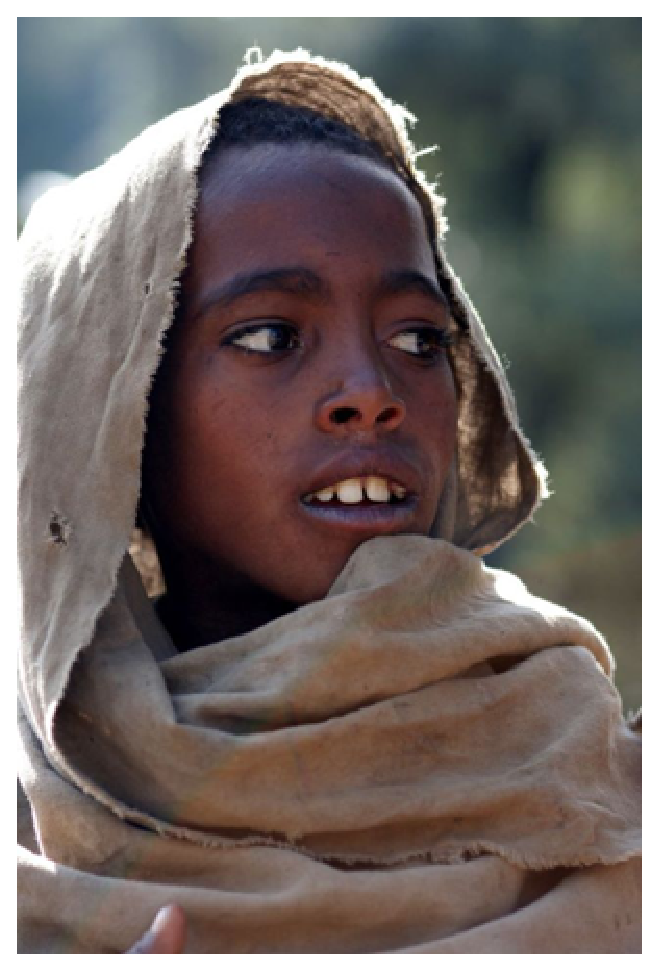
\includegraphics{imgs/etiopan.eps}}
	\scalebox{0.35}{\reflectbox{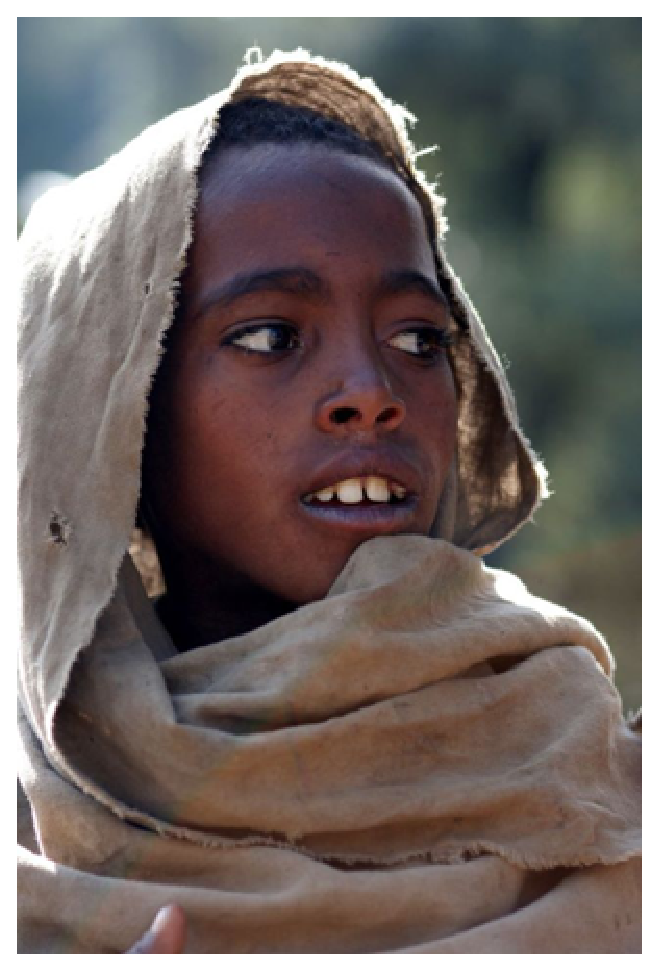
\includegraphics{imgs/etiopan.eps}}}
	\caption{Malý etiopánek a jeho bratříček}
	\label{pic:1}
	\end{figure}
\newpage

Rozdíl mezi vektorovým \dots
\begin{figure}[h]	% h means place the figure here
	\centering % center
	\scalebox{0.4}{
\includegraphics{imgs/oniisan.eps}}
	\caption{Vektorový obrázek}
	\label{pic:2}
\end{figure}\\

\dots a bitmapovým obrázkem
\begin{figure}[h]	% h means place the figure here
	\centering % center
	\scalebox{0.6}{
\includegraphics{imgs/oniisan2.eps}}
	\caption{Bitmapový obrázek}
	\label{pic:3}
\end{figure}

se projeví například při zvětšení. 

Odkazy (nejen ty) na obrázky \ref{pic:1}, \ref{pic:2} a \ref{pic:3}, na tabulky
\ref{tab:1} a \ref{tab:2} a také na algoritmus \ref{alg:1} jsou udělány pomocí
křížových odkazů. Pak je ovšem potřeba zdrojový soubor přeložit dvakrát.

Vektorové obrázky lze vytvořit i přímo v~\LaTeX u, například pomocí prostředí
\verb|picture|. Všechny rozměry jsou uváděny v~mm.

\begin{figure}
	\begin{center}
		\setlength{\unitlength}{1.35mm}
		\begin{picture}(115,158.5)
			\put(0,0){\linethickness{1pt}\framebox(115,158.5){}}

			\put(88,151.25){\vector(0,1){7.25}}
			\put(88,151.25){\vector(0,-1){7.25}}
			\put(90,144){\makebox(15,14.5){\shortstack{Výška\\ mezery\,=\,14,5}}}
			\put(88,139){\vector(0,1){5}}
			\put(88,139){\vector(0,-1){5}}
			\put(89,132){\makebox(15,14.5){\shortstack{Výška\\ mezery\,=\,10}}}
			\put(88,129){\vector(0,1){5}}
			\put(88,129){\vector(0,-1){5}}
			\put(89,122){\makebox(15,14.5){\shortstack{Výška\\ hlavièky\,=\,10}}}
			\put(88,117){\vector(0,1){7}}
			\put(88,117){\vector(0,-1){7}}
			\put(89,110){\makebox(15,14.5){\shortstack{Výška\\ mezery\,=\,14}}}
			\put(88,72.5){\vector(0,1){37.5}}
			\put(88,72.5){\vector(0,-1){37.5}}
			\put(89,55){\makebox(15,14.5){\shortstack{Výška\\ tìla\,=\,75}}}
			\put(88,27.5){\vector(0,1){7.5}}
			\put(88,27.5){\vector(0,-1){7.5}}
			\put(89,17){\makebox(15,14.5){\shortstack{Výška\\ mezery\,=\,15}}}
			\put(88,15){\vector(0,1){5}}
			\put(88,15){\vector(0,-1){5}}
			\put(89,4){\makebox(15,14.5){\shortstack{Výška\\ paty\,=\,10}}}

			\put(94.5,77){\linethickness{1pt}\framebox(15,10){\textbf{\shortstack{Okrajová\\ poznámka}}}}
			\put(88,96.5){\makebox(20,14.5){\shortstack{Mezera\,=\,9}}}
			\put(96,102){\vector(-1,-2){6}}
			\put(90,90){\vector(-1,0){4.5}}
			\put(90,90){\vector(1,0){4.5}}
			\put(92,87){\makebox(20,14.5){\shortstack{Šířka\\ boxu\,=\,15}}}
			\put(102,90){\vector(-1,0){7.5}}
			\put(102,90){\vector(1,0){7.5}}

			\put(94,43){\makebox(15,14.5){\shortstack{Výška\\ stránky\,=\,158,5}}}
			\put(102,55){\vector(1,1){10}}

			\put(112,79.25){\vector(0,1){79.25}}
			\put(112,79.25){\vector(0,-1){79.25}}

			\put(57.5,3){\vector(1,0){57.5}}
			\put(57.5,3){\vector(-1,0){57.5}}
			\put(52,3){\makebox(10,5){\shortstack{Šířka stránky = 115}}}

			\multiput(15,151.5)(0,-10){16}{\line(0,1){7}}
			\multiput(0,144)(10,0){11}{\line(1,0){7}}

			\put(7.5,90){\vector(1,0){7.5}}
			\put(7.5,90){\vector(-1,0){7.5}}
			\put(2.5,90){\makebox(10,5){\shortstack{Mezera = 15}}}

			\put(58,137){\vector(1,0){27.5}}
			\put(58,137){\vector(-1,0){27.5}}
			\put(55,137){\makebox(10,5){\shortstack{šířka boxu = 55}}}
			\put(30.5,124){\linethickness{1pt}\framebox(55,10){\textbf{Hlavièka}}}

			\put(30.5,35){\linethickness{1pt}\framebox(55,75){\textbf{Textové tìlo}}}

			\put(30.5,10){\linethickness{1pt}\framebox(55,10){\textbf{Pata}}}
		\end{picture}
		\caption{Vektorový obrázek v~prostøedí \texttt{picture}}
	\end{center}
\end{figure}

\end{document}
